
\section{Enigma}
\subsection{Opdracht}
De vierde ciphertekst was versleuteld met Enigma. Eerst implementeerden we een volledige Enigma machine. Daarna gingen we op zoek naar de gebruikte rotoren en hun beginstand.

\subsection{Een beetje extra onderzoek}
Voor we aan het kraken van enigma begonnen hebben we eerst het internet nog gebruikt om wat extra informatie te verzamelen. Deze info en de nota's van de les stelden ons in staat om de tekst relatief eenvoudig te kraken.
Hieronder een korte oplijsting met de belangrijkste bronnen van informatie die we gebruikten om meer te leren over Enigma, de geschiedenis en het kraken.

\begin{itemize}
\item \url{https://www.youtube.com/watch?v=G2_Q9FoD-oQ} \\
	Een video over de werking van Enigma, de internals, het elektrisch circuit ed.
\item \url{https://www.youtube.com/watch?v=d2NWPG2gB_A}
\url{https://www.youtube.com/watch?v=kj_7Jc1mS9k}
Een iets meer in depth gesprek over de geschiedenis van Enigma en de handelingen in Bletchley park.
\item De Wikipediapagina's over Enigma en Alan Turing
	\begin{itemize}
		\item \url{http://en.wikipedia.org/wiki/Alan_Turing}
		\item \url{http://en.wikipedia.org/wiki/Enigma_machine}
	\end{itemize}
	\item \url{http://www.bletchleypark.org.uk/content/hist/} \\ De Pagina van Bletchley Park met een heel stuk geschiedenis rond Enigma.
\end{itemize}


\subsection{Maken van de Enigma machine}
Eerste stap om Enigma te kunnen ontcijferen was om een werkende Enigma machine te maken. Als taal kozen we voor Go, omdat deze het heel eenvoudig maakt om concurrent functies uit te voeren. Op deze manier zouden we verschillende rotorposities tegelijk kunnen proberen, net als "The Bombe" dit deed in Wereldoorlog II. De implementatie was niet zo moeilijk; met de info die we hadden uit de les konden we eenvoudig de verschillende componenten implementeren: Rotor, Reflector en Plugboard. Voor elk van deze componenten schreven we testen zodat we zeker waren dat er geen fouten inzaten voor we ze samenbrachten in de Enigma klasse. Deze zorgde voor het linken van de componenten: elk character wordt naar de componenten gestuurd en output wordt geconcateneerd tot de ge\"encrypteerde of decrypteerde tekst. Om de volledige machine eenvoudig te kunnen gebruiken hebben we een JSON parser toegevoegd die een JSON file neemt en uit de info in deze file een Enigma construeert. Voorbeeldfiles zijn te vinden in de map jsonConfigFiles. Om de machine te testen encrypteerden we enkele teksten via de webapp\footnote{\url{http://www.algebra.ua.ac.be/stijn/enigma.phtml}}. Dit gaf telkens hetzelfde resultaat als onze implementatie.

\subsection{Crib graph en begin positie van de rotors}
Er was een crib gegeven, dus we konden makkelijk een crib graph opstellen. Hiervoor stelden we manueel een .dot file op, waarmee we een visuele voorstelling genereerden. Deze is hieronder weergegeven. \\
\begin{center}
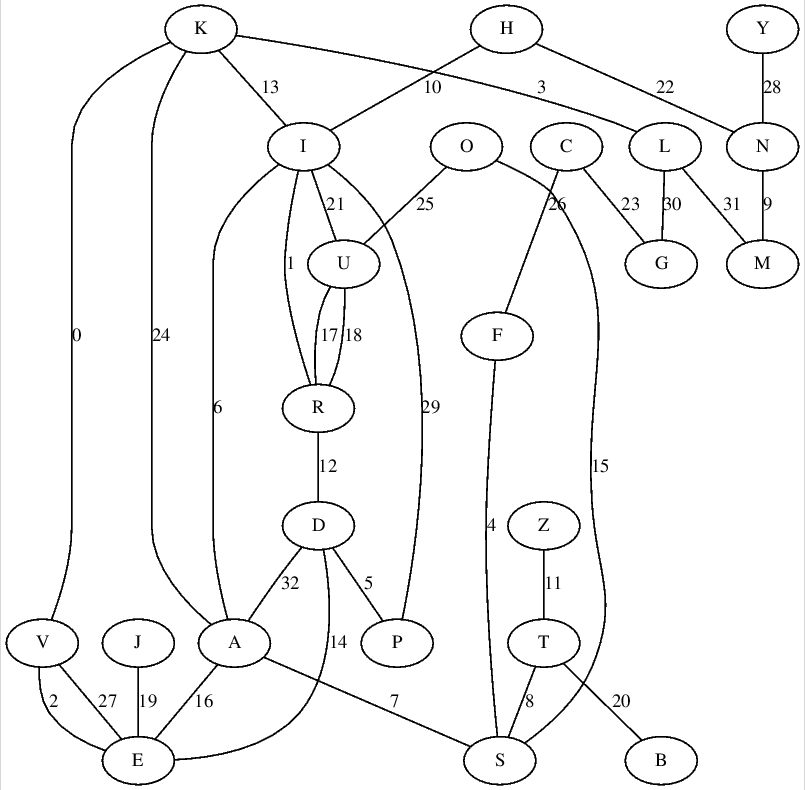
\includegraphics[scale=0.25]{enigma/graph.png}
\end{center}
Aan de hand van de graph konden we op zoek naar gesloten paden. Door de lengte van de crib waren er heel wat mogelijkheden. We bepaalden voor de letter U 6 gesloten paden. We gingen dan, met elke mogelijke volgorde van rotoren, op zoek naar een k waarvoor een letter invariant bleef op elk van die paden. Hiervoor was een kleine modificatie aan onze ge\"implementeerde Engima machine voldoende. We vonden dat er hiervoor slechts \'e\'en optie was, namelijk rotorvolgorde 420 met als beginstand KSY. De invariante letter was hier de U, wat betekent dat de U door het plugboard niet aangepast wordt. We herhaalden deze test met de letters A, D en I, waarvoor we ook telkens 5 \`a 6 gesloten paden zochten. Hier vonden we ook telkens slechts 1 of 2 resultaten, waaronder altijd \textbf{rotorvolgorde 420} met \textbf{beginstand KSY}. Dit was dus zeker het juiste antwoord. Uit deze resultaten vonden we ook dat het plugboard I en Y verwisselt, en de A en de D niet aanpast. Nu moesten we enkel nog op zoek naar de rest van het plugboard.

\subsection{Bepalen van het plugboard en ontcijferen van de tekst}
Omdat we een behoorlijk grote crib hadden, waren er voor de meeste letters gesloten paden te vinden in de graph. We konden dus gewoon een versimpelde versie van de voorgaande code draaien voor elke letter met gesloten paden om het plugboard verder te bepalen. Hiervoor hoefden we de test enkel voor de correcte rotorvolgorde en beginstand draaien. De enige letters zonder gesloten paden waren B, J, Q, T, W, X, Y en Z waarbij Q, W en X helemaal niet in de graph voorkwamen, en we al wisten dat Y met I werd omgewisseld. We vonden toch de mappings voor B, Q, W en Z omdat ze elk verwisseld werden met een letter die wel gesloten paden had. We hadden het plugboard dus op J, T en X na bepaald. Er waren nu echter maar 4 mogelijke plugboards over: ofwel werden twee van de drie letters met elkaar gewisseld ofwel werd geen enkele gewisseld. Door de ciphertekst met elk van de vier opties te decipheren, vonden we dat enkel die waarbij J, T en X niet werden aangepast de crib juist ontcijferde en dus juist was. Hiermee hadden we ook het plugboard volledig bepaald en konden we de tekst volledig ontcijferen. Het was een deel uit Die Blechtrommel van G\"unter Grass \footnote{\url{http://www.lawrenceglatz.com/germ3230/texte/grass1.htm}}.



